\documentclass{article}
\usepackage[utf8]{inputenc}

\usepackage{amsmath}
\usepackage{graphicx}
\usepackage{xcolor}
\usepackage[export]{adjustbox}[2011/08/13]
\usepackage{float}
\usepackage{hyperref}
\usepackage{setspace}
\usepackage{fullpage}

\hypersetup{colorlinks=true}

% shortcuts for covariant basis vectors
\newcommand{\er}{{\mathbf e}_{\rho}}
\newcommand{\ev}{{\mathbf e}_{\vartheta}}
\newcommand{\ez}{{\mathbf e}_{\zeta}}

\bibliographystyle{ieeetr}

\title{APC 524 Design Document}
\author{Daniel Dudt, Dario Panici, Evan Yerger}
\date{December 15, 2020}

\begin{document}

\maketitle

\section{Background}

\subsection{Motivation}

Determining the equilibrium of a plasma is crucial for the design and operation of magnetic confinement fusion reactors.
Equilibrium calculations are used for understanding basic plasma physics, interpreting diagnostic data from experiments, running real-time control systems to stabilize the plasma, and for optimizing the design of future machines.
Most mainstream magnetic confinement concepts for controlled fusion involve toroidal reactors, such as the tokamak and stellarator.
The tokamak is characterized by toroidal symmetry, while the stellarator does not have an ignorable coordinate and is fully ``three-dimensional''.
The nonlinear partial differential equations that describe an equilibrium are computationally challenging to solve, especially for the complicated geometries of stellarators.
Existing codes such as VMEC \cite{Hirshman1983} are expensive to run and do not always converge to the desired result, making them poorly equipped for future progress.
DESC \cite{Dudt2020} is a modern code designed to meet the increasing demands of advanced stellarator performance, and the goal of this project is to make significant contributions to the development of DESC.

\subsection{Theory}

Ideal magnetohydrodynamics (MHD) is a single-fluid model of plasma.
It describes the equilibrium of a static plasma through a force balance equation, along with Amp\`ere's and Gauss's laws:
%
\begin{subequations}
  \label{eq:equil}
  \begin{align}
    \label{eq:momentum}
    \mathbf{J} \times \mathbf{B} &= \nabla p \\
    \label{eq:Ampere}
    \nabla \times \mathbf{B} &= \mu_0 \mathbf{J} \\
    \label{eq:Gauss}
    \nabla \cdot \mathbf{B} &= 0.
  \end{align}
\end{subequations}
%
Here $\mathbf{J}$ is the current density, $\mathbf{B}$ is the magnetic field, $p$ is the plasma pressure, and $\mu_0$ is the magnetic constant.
Combining the force balance (\ref{eq:momentum}) and  Amp\`ere's Law (\ref{eq:Ampere}), a force balance error $\mathbf{F}$ can be defined as
%
\begin{equation}
  \label{eq:F}
  \mathbf{F} \equiv \frac{1}{\mu_0} \left( \nabla \times \mathbf{B} \right) \times \mathbf{B} - \nabla p = F_\rho \nabla\rho + F_\beta \mathbf{\beta} = \mathbf{0}
\end{equation}
%
where $\mathbf{\beta} \equiv B^\zeta \nabla \vartheta - B^\vartheta \nabla \zeta$.
The flux coordinate system $(\rho,\vartheta,\zeta)$ is a specific choice that makes the magnetic field lines ``appear straight'' to simplify calculations, and is related to the usual toroidal coordinates $(R,\phi,Z)$ as shown in Figure \ref{fig:coords}.
Equation (\ref{eq:F}) is a system of nonlinear partial differential equations (PDEs) and it must be satisfied throughout the entire plasma volume when in equilibrium.
Using Gauss's law (\ref{eq:Gauss}) and assuming that nested flux surfaces exist $\mathbf{B}\cdot\nabla\rho=B^\rho=0$, the magnetic field can be expressed in the following contravariant form of the flux coordinate system $(\rho,\vartheta,\zeta)$:
%
\begin{equation}
  \label{eq:B}
  \mathbf{B} = B^\vartheta \ev + B^\zeta \ez = \frac{\partial_\rho \Psi}{2\pi \sqrt{g}} \left( \iota \ev + \ez \right).
\end{equation}
%
Here $\Psi$ is the toroidal magnetic flux and $\iota\equiv d\vartheta/d\zeta = B^\vartheta/B^\zeta$ is the rotational transform.
The covariant basis vectors $\ev$ and $\ez$ and the jacobian of the coordinate system $\sqrt{g}$ are known from the shapes of the flux surfaces: $R(\rho,\vartheta,\zeta)$ and $Z(\rho,\vartheta,\zeta)$.
Solving the force balance given in (\ref{eq:F}) subject to a magnetic field of the form given in (\ref{eq:B}) will satisfy all of the MHD equilibrium conditions provided in (\ref{eq:equil}).
The actual scalar equations that get minimized are
%
\begin{subequations}
  \label{eq:f}
  \begin{align}
    f_\rho(R,Z) &= F_\rho \lVert\nabla\rho\rVert_2 \sqrt{g} \Delta\rho\Delta\vartheta\Delta\zeta \text{sign}\left(\nabla\rho\cdot\er\right) \\
    f_\beta(R,Z) &= F_\beta \lVert\mathbf{\beta}\rVert_2 \sqrt{g} \Delta\rho\Delta\vartheta\Delta\zeta \text{sign}\left(\mathbf{\beta}\cdot\ev\right) \text{sign}\left(\mathbf{\beta}\cdot\ez\right)
  \end{align}
\end{subequations}
%
along with additional equations to enforce the boundary conditions.
This is known as an ``inverse formulation'' because the toroidal coordinates are solved for in terms of the flux coordinates, which are treated as the independent variables.
Calculating the equilibrium magnetic field is equivalent to determining the transformation between these two coordinate systems.

The PDEs are discretized using pseudospectral methods.
The flux surfaces are represented by the coefficients of a global Fourier-Zernike basis set of the form:
%
\begin{subequations}
	\begin{align}
	\label{eq:R_basis}
	R(\rho,\vartheta,\zeta) &= \sum_{n=-N}^{N} \sum_{m=-M}^{M} \sum_{l\in L} R_{lmn} \mathcal{Z}^{m}_{l}(\rho,\vartheta) \mathcal{F}^{n}(\zeta) \\
	\label{eq:Z_basis}
	Z(\rho,\vartheta,\zeta) &= \sum_{n=-N}^{N} \sum_{m=-M}^{M} \sum_{l\in L} Z_{lmn} \mathcal{Z}^{m}_{l}(\rho,\vartheta) \mathcal{F}^{n}(\zeta)
	\end{align}
\end{subequations}
%
where $\mathcal{Z}^{m}_{l}$ is the Zernike polynomial with radial mode $l$ and azimuthal mode $m$, $\mathcal{F}^{n}$ is a Fourier component with wave number $n$, and $L = |m|, |m|+2, |m|+4, \ldots, 2 M - |m|$.
From the state vector of coefficients $\mathbf{x} = [R_{lmn}, Z_{lmn}]^T$, the values and partial derivatives of $R(\rho,\vartheta,\zeta)$ and $Z(\rho,\vartheta,\zeta)$ are transformed to physical space at a set of collocation points.
All of the nonlinear calculations involved to compute (\ref{eq:f}) are performed in physical space at these nodes, resulting in a residual vector $\mathbf{f} = [f_\rho, f_\beta]^T$.
Starting from an initial guess, DESC computes the equilibrium solution by finding the flux surface geometry that minimize these errors on a given grid of collocation points: $\mathbf{f}(\mathbf{x}) \approx \mathbf{0}$.
This optimization process is performed with a quasi-Newton method, and will be referred to as the ``inner loop'' of the DESC algorithm.
The ``outer loop'' performs a sequence of these optimizations with different input parameters, and can perturb the previous solution to give a good initial guess for the next optimization step with the new inputs.
For example, this outer loop can be used to increase the numerical resolution from a crude initial solution to one with many spectral modes.
Another application is to perform scans in solution space over a physics parameter such as pressure, by starting from a vacuum solution and then solving for the equilibrium at increasingly higher pressures.

\begin{figure}
	\centering
	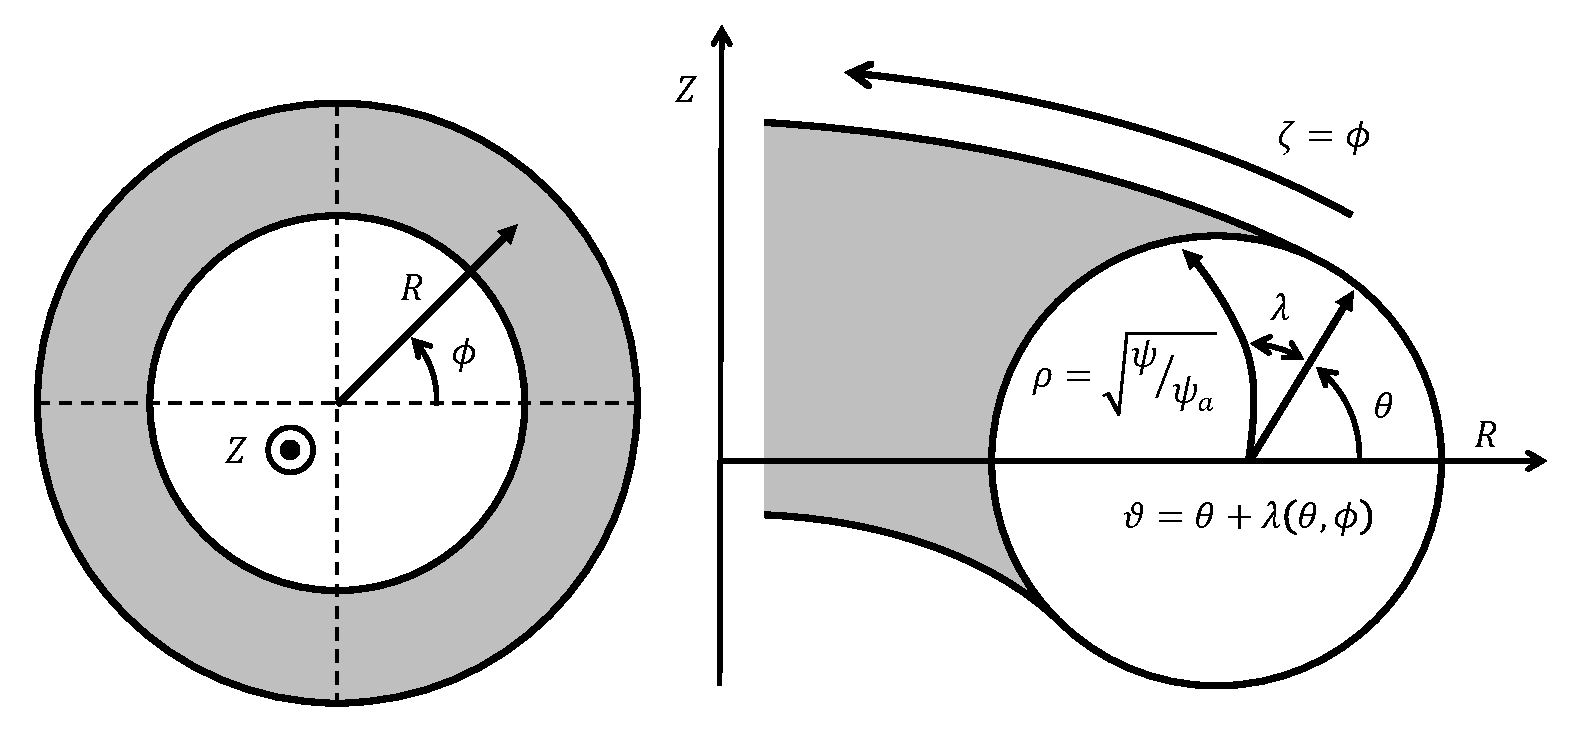
\includegraphics[width=0.8\linewidth,center]{./figs/coordinates.pdf}
	\caption{Toroidal coordinate system $(R,\phi,Z)$ and the flux coordinates $(\rho,\vartheta,\zeta)$.}
	\label{fig:coords}
\end{figure}

\section{Project Goals}

\subsection{Initial State}

Before undertaking this project, DESC already existed as an open-source Python software package.
The user interface was to create an input file detailing all of the solver parameters, and then pass that input file as a command line argument.
The user could also pass flags to plot the results, but this output was only preset routines without much opportunity for customization.
Internally, the DESC algorithm was implemented sequentially with a functional rather than class structure.
Although the functions were well documented, each had a unique call signature and there was a lack of a common interface between different parts of the code.
New features were added to the code by creating another option in the input file format, and handling the new cases with if-else logic in the main driver script.

DESC relies on other software packages to outsource some functionality.
The NumPy \cite{NumPy} library is used to handle and vectorize all array operations in the system of equations.
Initially, all of the optimization routines for the inner loop were provided by the SciPy \cite{SciPy} optimization library.
Many of these routines rely on information of how the objective function changes with respect to state variables, which is encoded in the Jacobian matrix $\frac{\partial\mathbf{f}}{\partial\mathbf{x}}$.
This information is also needed to perform the outer loop perturbations, so it is important for DESC to compute the Jacobian matrix quickly and accurately.
This is accomplished with the use of JAX \cite{JAX}, an open source machine learning package for Python.
JAX provides automatic differentiation of arbitrary Python functions by overloading NumPy operations, as well as just-in-time (JIT) compilation and optimization for speed-up on repeated function calls.
It also allows for operations to be computed on a GPU, which can greatly accelerate the matrix-vector operations necessary for the optimization algorithm.
The initial state of the code had JAX implemented, but was disorganized about when it should be used over regular NumPy operations.

\subsection{Goals}

While DESC was functional in its initial state, it did not have a unified or high-level class structure organization to it.
It also was not extensively covered by testing, had not been thoroughly profiled for speed optimization, and lacked certain features that would make it more useful to the user.
With those shortcoming in mind, the aim of this project was to improve DESC in the following ways:
%
\begin{enumerate}
\item Refactor the code into a modular class structure
\item Expand the coverage of the existing testing suite
\item Profile the code to identify bottlenecks and explore optimization options
\item Extend the plotting capabilities to provide more solution visualization capabilities
\end{enumerate}

As mentioned in the previous section, the previous version of DESC had very minimal class structure.
This resulted in cumbersome control logic and unclear interfaces between different parts of the code.
Our primary goal of this project is to refactor DESC into a class structure that takes advantage of object-oriented programming.
This improvement will streamline the code and provide a consistent application programming interface (API) for adding new functionality as users expand the software to meet additional applications.
The new modularity will also make it easier to perform unit testing to ensure that the code is implemented properly and returns the desired output.
The existing continuous integration (CI) automated testing suite only covered 22\% of the DESC code, and our goal was to increase this converage to over 50\%.
Computational efficiency is also essential for DESC, since it was developed in the hope of finding stellarator equilibria faster than other codes.
Once the major refactoring was complete, we planned to profile the code to identify the bottlenecks and pursue any opportunities for optimization.
Finally, we also intended to create a class responsible for plotting 
Accurate solutions are only useful if they can be viewed, and the goal of this effort was to provide the user with a more flexible and interactive analysis tool.

\section{Design}

\subsection{Original Design Plan}

The organizational structure is shown in the class diagram in Figure \ref{fig:uml}.
%
\begin{figure}[H]
  \centering
  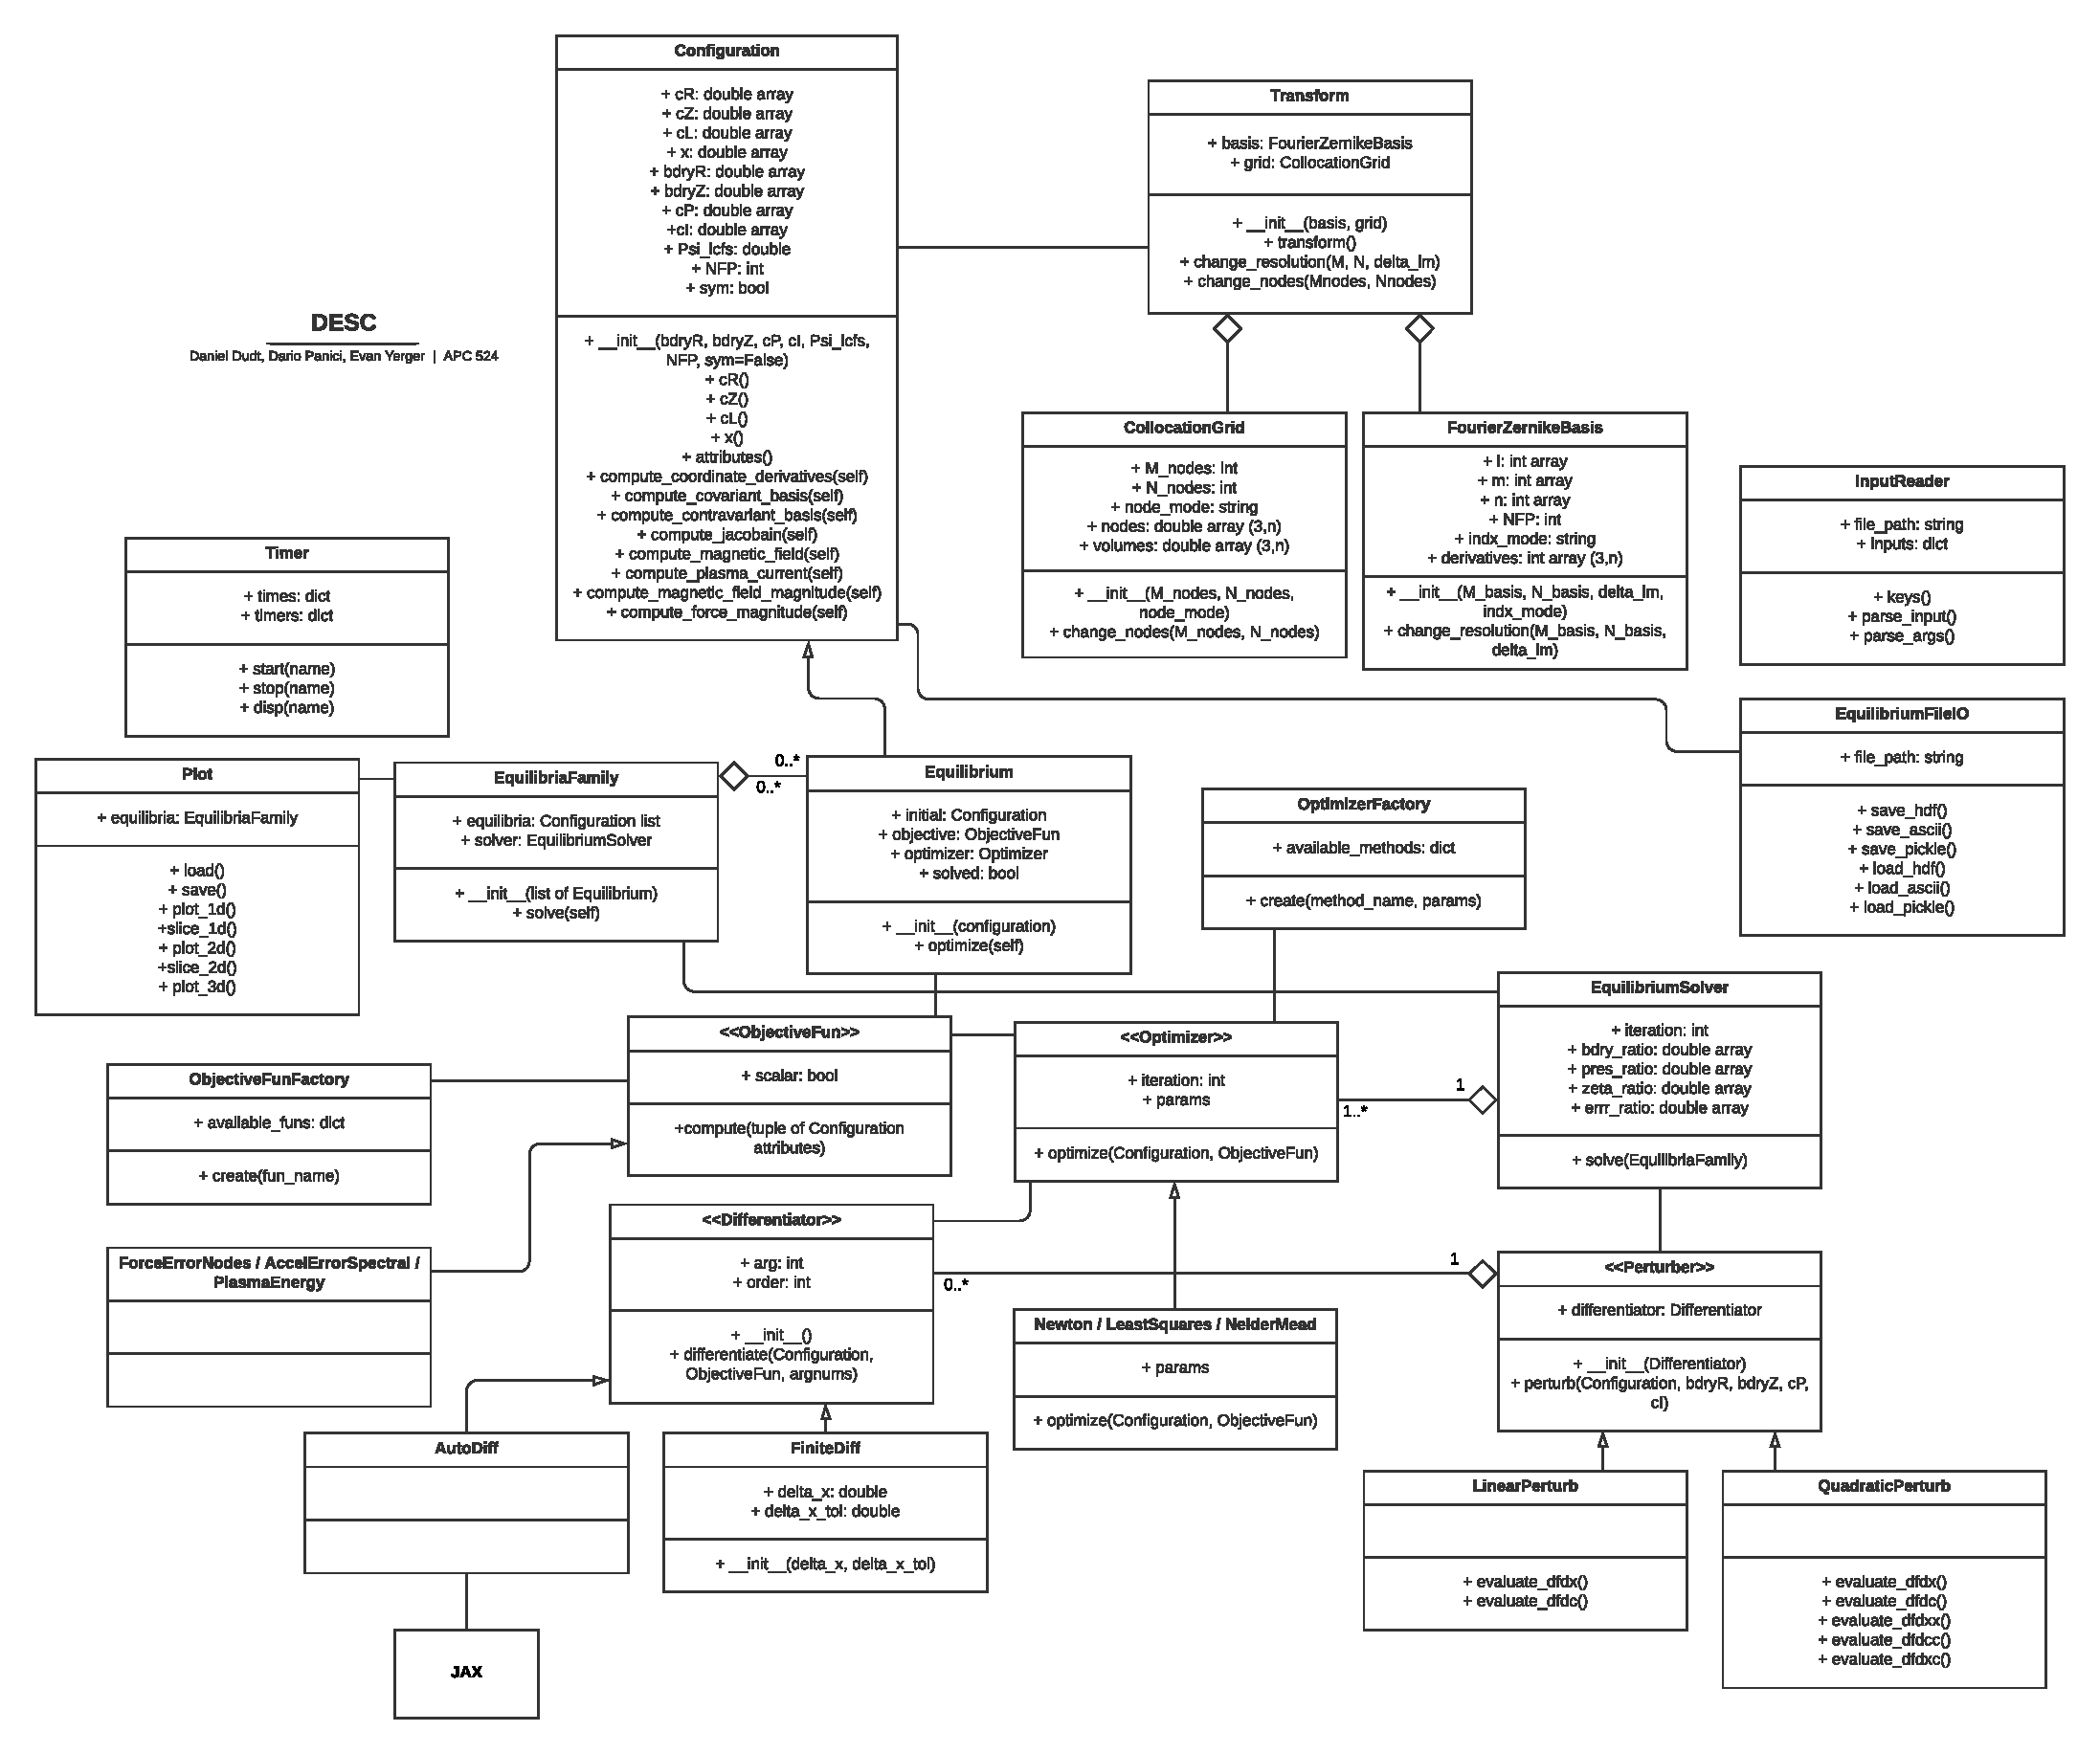
\includegraphics[width=1.6\linewidth,center]{./figs/UML_06.pdf}
  \caption{Class Diagram}
  \label{fig:uml}
\end{figure}

The interface is generally split into two parts: one computes an equilibrium from command line arguments; the other to plot solutions from saved files (generated by the solver).
When calculating a solution, the user must call the program with the input filename as an argument. Other optional arguments may be included and are detailed in the existing documentation.
The command line arguments and input file are parsed, and the required instances of the class objects will be created in order to solve.
A solution algorithm is called as a method of the EquilibriaFamily class, which creates new Equilibrium objects inside of it and saves aspects of the solution to the output file, as well as uses the linked EquilibriumSolver object to solve the problem.
Once a solution has been found and an output file saved, user can instantiate a Plot class with the name of the output file.
Then methods of this class would be called to plot specified parts of the solution (magnetic field, flux surfaces, etc) for specified domains (1-D profiles, 2D plot at a given toroidal cross-section, etc) at specified iterations of the solution (default the final solution, but could plot initial or intermediate solutions).

Another envisioned use of the code is in an interactive sense, where a user could in a script instantiate an Equilibrium and an EquilibriaFamily from an input file, and from there use the solve method of EquilibriaFamily to solve from the initial guess through to the final Equilibrium at the desired resolution. In this way, the user can use the Plot class to visualize not only the final result at the desired resolution, but also to see intermediate solutions (located as earlier Equilibrium objects inside of EquilibriaFamily) as the outer solving loop progressively stepped up the resolution of the solution.

\subsection{Final Implementation}

While the refactored project largely follows the original design plan, we made a number of changes made during development.
One such change was to the Equilibrium\_IO class, which is no longer a class, but a collection of classes.
In order to resolve a circular import error, the IO either had to be fully agnostic of the objects it was saving and loading, or it had to have save and load functions specific to each object.
In the former case, each object would need its own save and load functions, but the IO would have a homogeneous user interface across all objects; the later required that the user remember or look up functions unique to each object.
We decided that for reasons of a simpler interface and greater flexibility for future expansion of the IO, the former approach would be used.
We also split Equilibrium\_IO into a number of abstract base classes: IO, Reader, and Writer.
This had a number of benefits, including an increase in the overall flexibility of the code, a reduction in the amount of code reproduction necessary for modifying the IO.
Adding a pickle format was as easy as creating a new subclass of IO called PickleIO which contained format-specific functions, and creating pickle Readers or Writers using a class that inherits from PickleIO and Reader or Writer, respectively.
This inheritance structure means that all IO objects must conform to a single interface, allowing the save and load functions of particular objects to be agnostic of the file format used.

%
\begin{figure}[H]
	\centering
	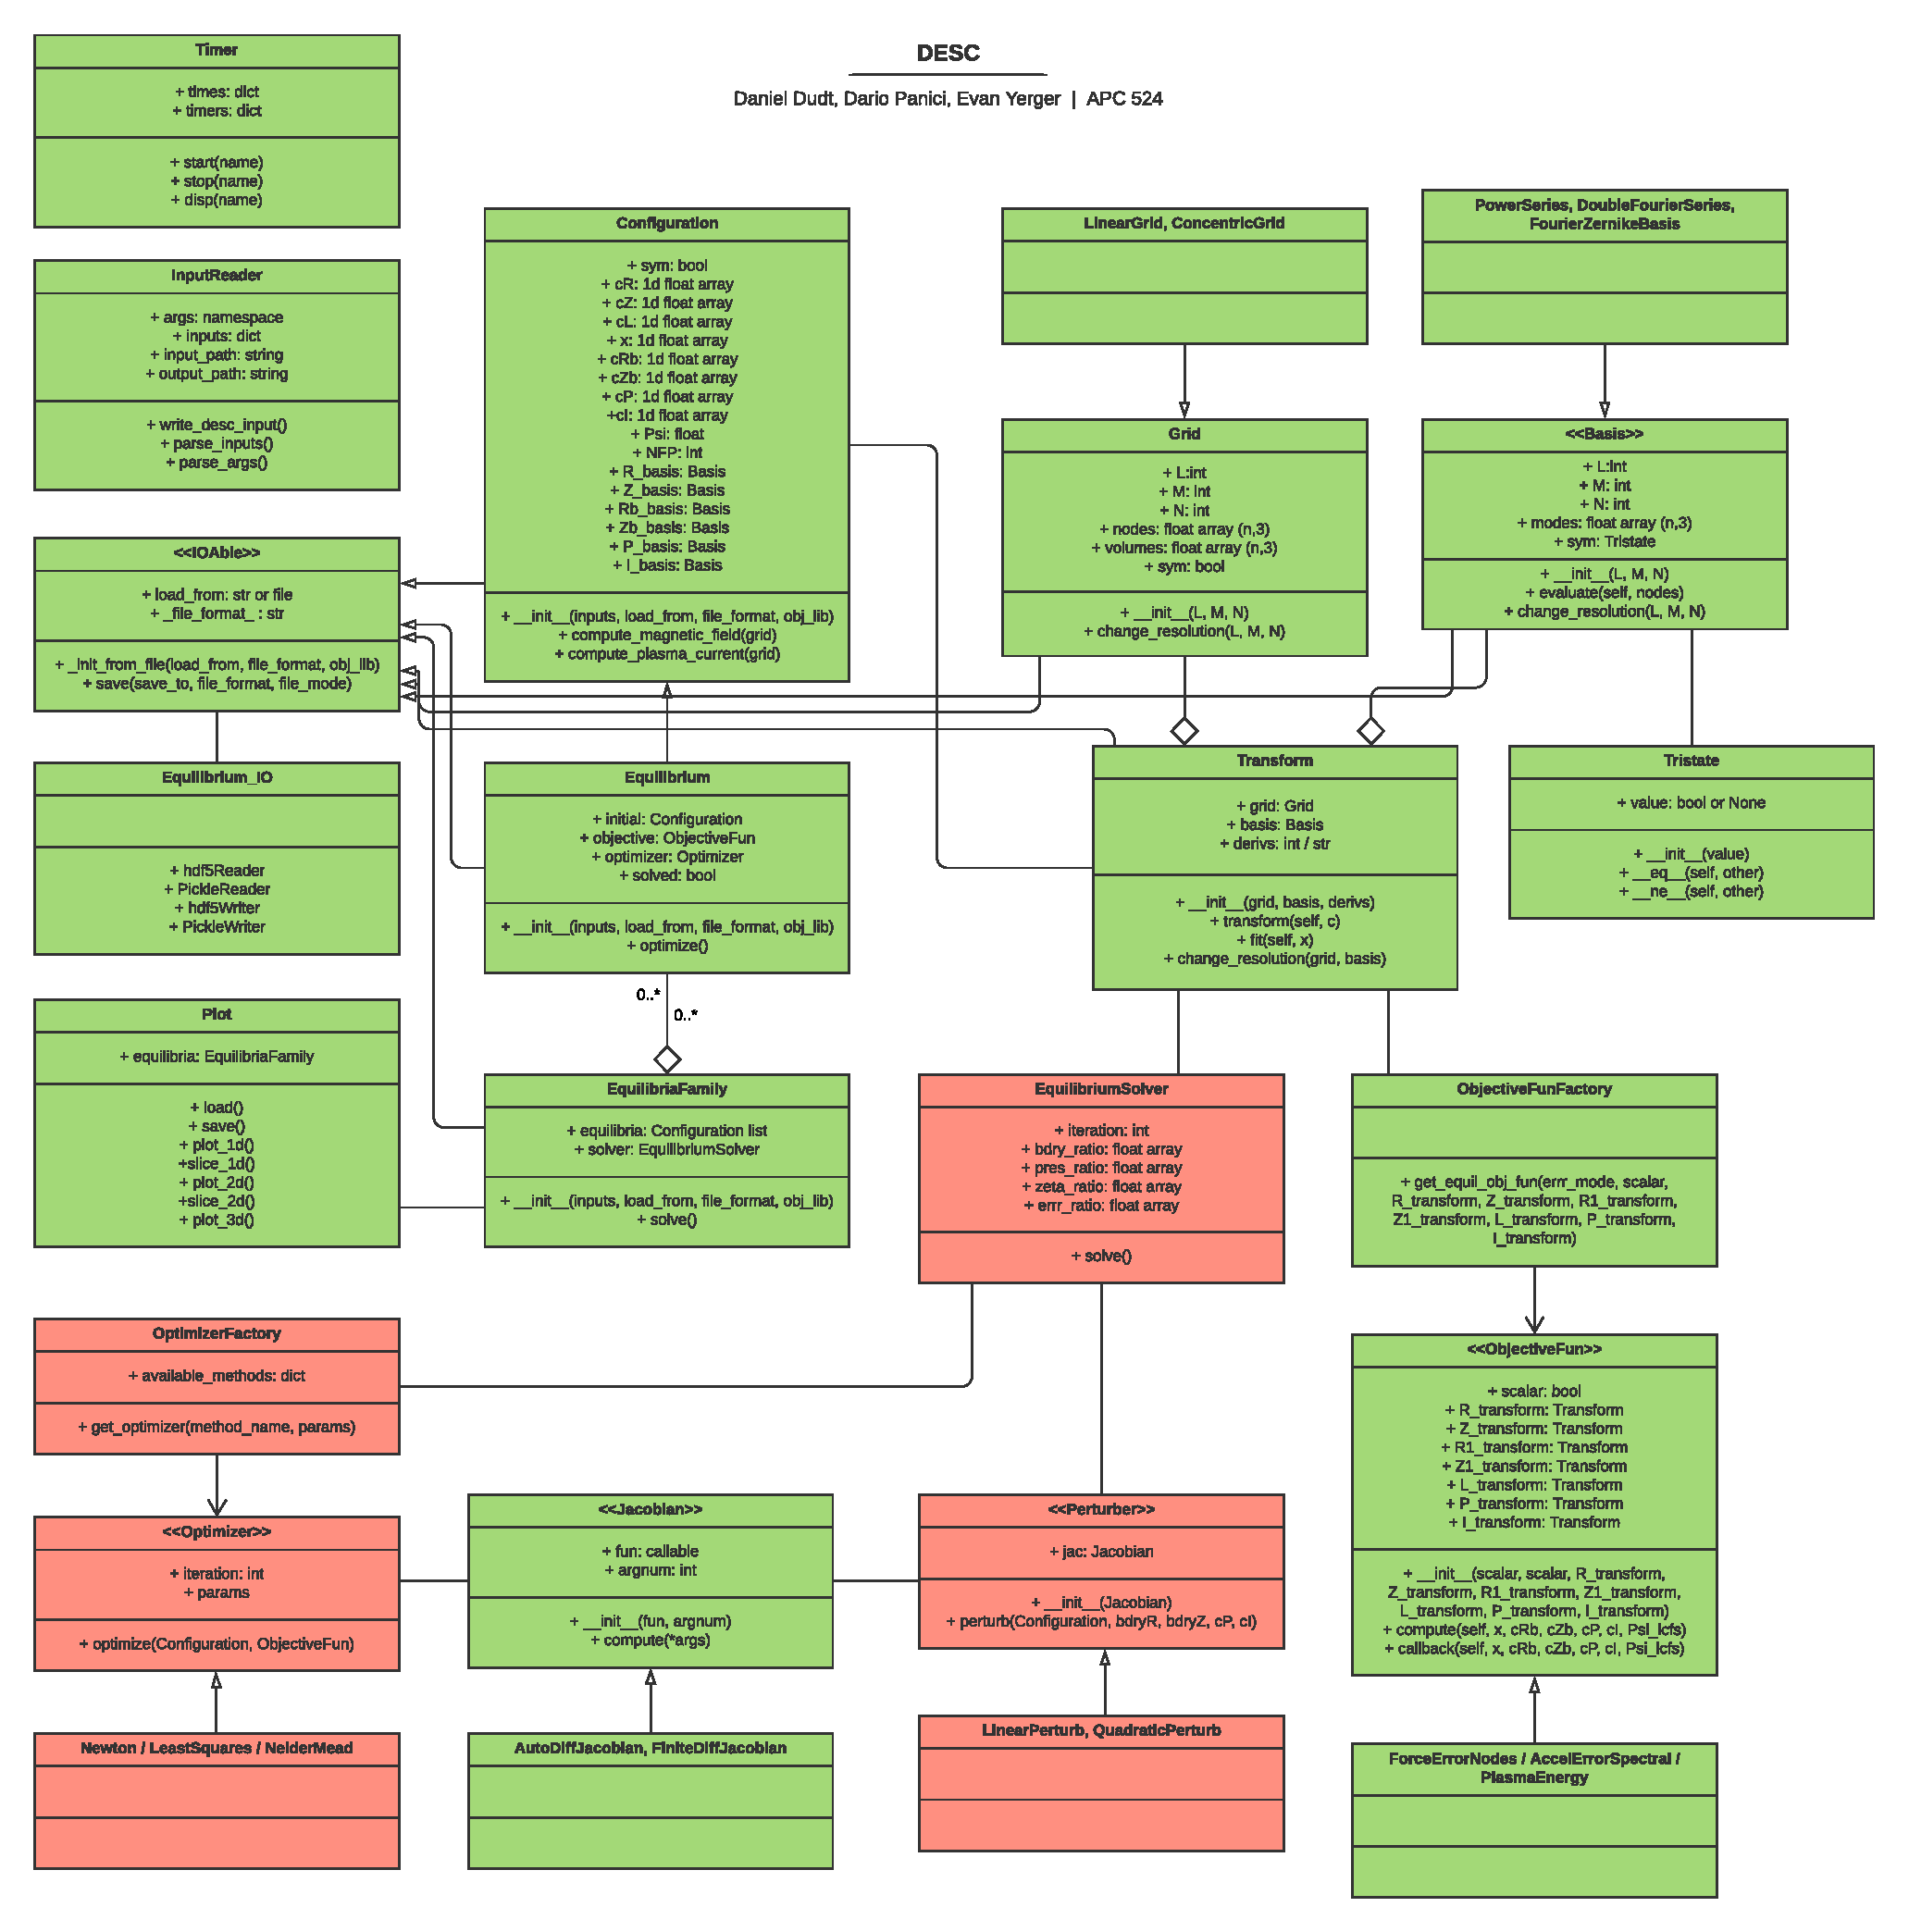
\includegraphics[width=1.6\linewidth,center]{./figs/DESC_UML.pdf}
	\caption{Class Diagram}
	\label{fig:UML}
\end{figure}


%
\begin{figure}[H]
	\centering
	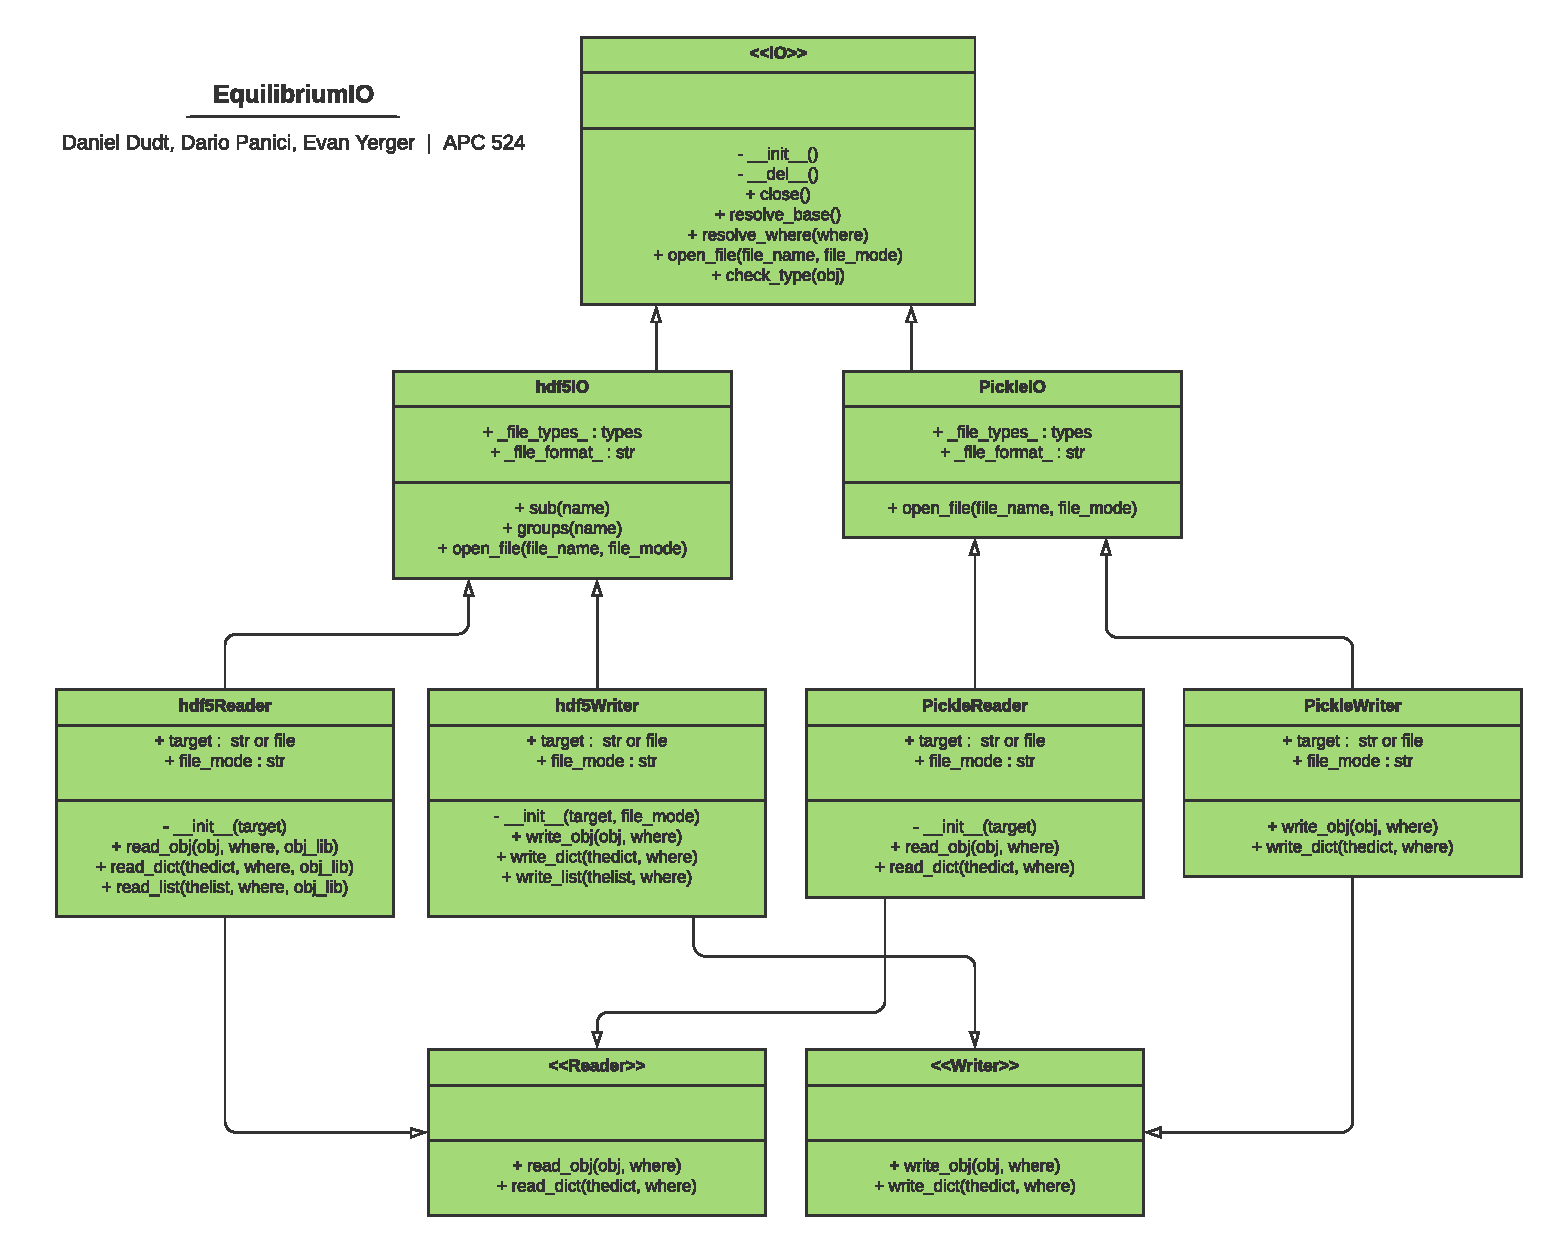
\includegraphics[width=1.6\linewidth,center]{./figs/EquilibriumIO_UML.pdf}
	\caption{IO}
	\label{fig:IO_UML}
\end{figure}

\section{Development Process}

\subsection{Git Workflow}

For our project, we decided to go with the git workflow that uses parallel dev and master branches.
The idea of the workflow is to branch from master to work on feature branches, then merge those to dev where the testing will take place.
Then, once tests are passed, the feature branch is merged to master.

This works well when the feature branches are all independent of eachother, so merge conflicts on dev are minimized.
However, in our project we were refactoring an existing code base and a lot of our feature branches had some sort of inter-dependence, especially at the start.
A case of this is in the creation of the Transform class that is used as the base class for the coordinates at which we evaluate our objective functions.
The Transform class is essentially the interface between the spectral coefficients that contain the information about an equilibrium and the real-space values like force and energy which we are actually minimizing.
We initially each made separate feature branches off of master with a defined refactoring task for each branch.
But, when it came time to bring the branches back into master, we realized that the Transform branch, where the Transform class was created and code refactored to work with it, touched many parts of the other branches' files.
This created a headache when it came time to merge Transform into dev, as not only merge conflicts had to be resolved, but also other working parts from other feature branches were broken.

How we ended up resolving this issue was to first merge the other, less broadly-changing feature branches into master.
Then, from the Transform branch, we cherry-picked the latest commits from master into Transform.
With this, we could then make the necessary changes to allow Transform to play nice with the other branch commits, while also keeping the dev branch strictly for testing and not for bug-fixing commits.
So, we were able to modify the other necessary parts of the code to allow it to run with the Transform class, and then ended up merging back to master.

From this, we learned that the parallel dev and master workflow works best when feature branches are smaller in scope, and are merged back to master often.
This way, any individual feature branch does not fall behind the master branch, and each feature branch can more easily be independent of eachother.

Another thing we learned as we worked in this workflow was the dev branch should be used only for testing.
Finding bugs on dev and then fixing them by committing code to dev seemed fine at first.
However, when we would go to make further changes on our feature branches, we would realize that some bug we fixed on dev is still present on the feature branch.
This would then require us to have to essentially re-commit the bug fix on the feature branch.
Finally when we wanted to test the feature branch by merging with dev before merging to master, we would encounter confusing merge conflicts due to having fixed the bug separately on dev and on the feature branch.
Thus, we learned the hard way that the dev branch should never be advanced alone, and instead should only be advanced by merging feature branches, and all work and fixes should be done on feaure branches to keep dev and the feature branches both up-to-date on bug fixes.

\subsection{Continuous Integration}

The continuous integration workflow with automated tested helped us catch bugs as new code was developed.
In our requirements file we initially listed support for the latest version of JAX, version 0.2.5.
JAX is still being actively developed and there have been major changes since the DESC code was first written.
When pushing changes to the new Transform structure that relies heavily on the use of jax.numpy arrays, the new changes were failing the tests on the virtual machines that were running JAX, but passing on our local computers without JAX.
This problem was puzzling, because JAX is intended to replicate most of the usual numpy operations.
Around the same time, an independent user of the code had also reported a problem with running JAX on the original DESC repository.
It turned out that some of the operations we were using were no longer supported in the newer version of JAX, and reducing the installation requirement to version 0.1.77 resolved the issue.
The lesson learned was that maintaining compatibility with other software packages can be laborsome, but frequent testing (from both automated tests and beta users) can help catch problems when they arise.

\section{Profiling Results}


As DESC is written in Python, we plan to use the Python profiling modules profile and cProfile to identify where the code spends most of its time. Once we have completed profiling the code, we will identify the routes we can take to optimize the performance of the code. This will necessarily depend on the results of the profiling, but some avenues we anticipate we could take is to parallelize any embarrasingly parallel tasks in the code to work across multiple CPUs. There are different tools we can use to do this, one route could be to utilize the parallel processing Python module multiprocessing, which allows for splitting tasks across multiple threads of a CPU. Additional possible optimization paths could relate to the GPU. Currently, the solution resolution possible running DESC and utilizing the GPU is limited by memory on the GPU, as the jacobian necessary for the optimization algorithm's computations on the GPU becomes larger than the memory on the GPU can handle. One possible way we can explore to remedy this is to split up the jacobian and evaluate parts of the computation on different GPUs in parallel, or on the same GPU but only in chunks at a time, and recover the full result on the CPU, to avoid GPU memory issues.


The actual evaluation time for all of these tests depends on the resolution used.  In this case, it was...

Talk about how the tests were not performed with JAX

%
\begin{figure}[H]
	\centering
	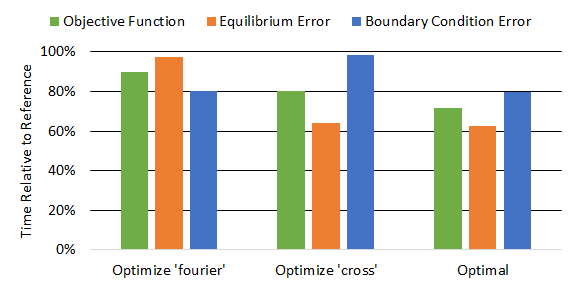
\includegraphics[width=0.6\linewidth,center]{./figs/compute_time_opt.png}
	\caption{Reduction in execution time to compute the equilibrium force balance objective function, relative to the original code, for different stages of optimization.}
	\label{fig:compute_opt}
\end{figure}
%
\begin{figure}[H]
	\centering
	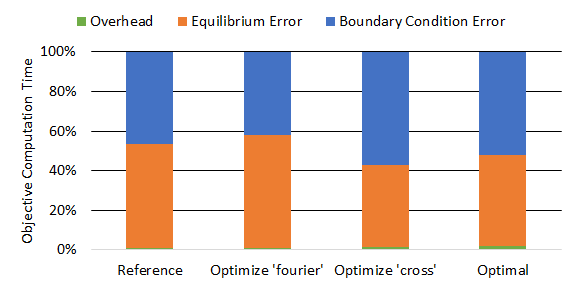
\includegraphics[width=0.6\linewidth,center]{./figs/compute_time_rel.png}
	\caption{Relative portion of time to compute the equilibrium force balance objective function spent in each subfunction, for different stages of optimization.}
	\label{fig:compute_opt}
\end{figure}
%
\begin{figure}[H]
	\centering
	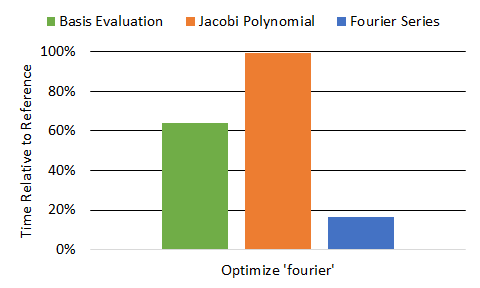
\includegraphics[width=0.6\linewidth,center]{./figs/compile_time_opt.png}
	\caption{Reduction in execution time to evaluate the Fourier-Zernike basis function, relative to the original code, for different stages of optimization.}
	\label{fig:compute_opt}
\end{figure}
%
\begin{figure}[H]
	\centering
	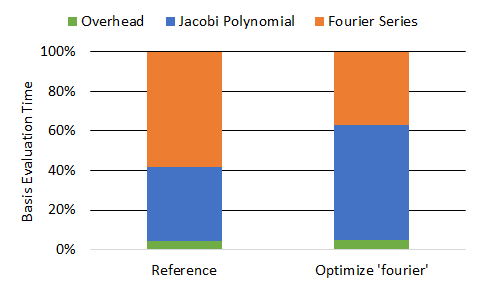
\includegraphics[width=0.6\linewidth,center]{./figs/compile_time_rel.png}
	\caption{Relative portion of time to evaluate the Fourier-Zernike basis function spent in each subfunction, for different stages of optimization.}
	\label{fig:compute_opt}
\end{figure}

\section{Future Work}

\subsection{Finish Realization of Object-Oriented Design}

The most immediate future work for this project would be to complete the refactoring of the code into an object-oriented design.
The main part of the code that remains in a functional implementation is the outer loop solver.
While the refactoring we completed did increase the legibility of the outer loop solver function, there are still aspects of it that would benefit from refactoring.
This would come in the form of creating the EquilibriumSolver and Optimizer classes from the UML diagram, inside of which would handle the logic of the inner-outer loop optimization algorithm.
We foresee the most difficulty in this task coming from deciding how to split the necessary steps and control logic across the respective objects.
For example, in the outer loop, a new Equilibrium must be created and perturbed, in order to then be sent into the inner optimization loop.
Should the EquilibriumSolver object be able to create new Equilibrium objects, even though it is not directly connected to an Equilibrium?
We have in our UML diagram an outline of what we think is the best way to approach this, but it is the concrete answers to these questions that we will need to decide in order to finish the implementation of our complete design.

\bibliography{sources}

\end{document}
